\documentclass[a4paper]{article}
%\usepackage{fourier-otf}
\usepackage[utf8]{inputenc}
\usepackage{graphicx}
\usepackage{algorithm}
\usepackage{algpseudocode}
\usepackage{float}
\usepackage{lipsum}
\usepackage{scrextend}
\usepackage{biblatex}
\addbibresource{bibliography.bib}
\usepackage{listings}
\usepackage{amsmath}
\usepackage{amsfonts}
%\usepackage[square,sort,comma,numbers]{natbib}
\newtheorem{theorem}{Theorem}[section]
\usepackage{color}
\usepackage{makeidx}
\usepackage{titlepic}
\definecolor{mygreen}{rgb}{0,0.6,0}
\definecolor{mygray}{rgb}{0.5,0.5,0.5}
\definecolor{mymauve}{rgb}{0.58,0,0.82}
\lstset{ %
	backgroundcolor=\color{white},   % choose the background color
	basicstyle=\footnotesize,        % size of fonts used for the code
	breaklines=true,                 % automatic line breaking only at whitespace
	captionpos=b,                    % sets the caption-position to bottom
	commentstyle=\color{mygreen},    % comment style
	escapeinside={\%*}{*)},          % if you want to add LaTeX within your code
	keywordstyle=\color{blue},       % keyword style
	stringstyle=\color{mymauve},     % string literal style
}
\usepackage{hyperref}
\hypersetup{
  colorlinks   = true,    % Colours links instead of ugly boxes
  urlcolor     = black,    % Colour for external hyperlinks
  linkcolor    = black,    % Colour of internal links
  citecolor    = black      % Colour of citations
}
%\title{First chapter}

%\author{F.Bernardi}

%\protect\\ 

\newcommand{\myName}{Fabrizio Bernardi}
\newcommand{\myTitle}{Modeling and data analysis of the calcium activity in somatostatin interneurons from in vivo imaging on mice }
\newcommand{\myDegree}{Programme: \protect\\ \textit{Mathematical Engineering}}
\newcommand{\myCycle}{XXXI cycle}
\newcommand{\myDepartment}{Department of Mathematics}
\newcommand{\myUni}{Politecnico di Milano}
\newcommand{\myYear}{2022}
\newcommand{\myTime}{01 Jan \myYear}

\pdfbookmark{Cover}{cover}

\begin{document}
	
	
	
\section{Mathematical modeling of neuron's electric activity}

In Section 1.1, the concept of \textit{excitability} of neurons has been introduced: neurons are able to generate and transmit \textbf{electrical impulses} as reaction to external stimuli. These impulses are a direct consequence of rapid changes in intracellular end extracellular \textit{ionic concentrations} of main elements such as $Na^+, Cl^-, K^+, Ca^{2+}$. The change in such concentrations determines a change in the potential crossed across the cell's membrane, and the formation of an \textbf{action potential}. \\
In this chapter, mathematical models to describe the behaviour of such quantities are presented. After having introduced the main assumptions of the model, the equivalent circuit formulation for cellular electryphyioslogy will be presented, along with different models to describe its electrical components. Finally, the main model to describe the propagation of the action potential between different neurons will be under study, namely the \textbf{cable equation model}. These models consist \textbf{ordinary differential equations (ODEs)} or \textbf{partial differential equations (PDEs)}, to be numerically solved through appropriate technqiues.

\subsection{Electrical activity in neurons}

\begin{figure}[H]
	\begin{center}
		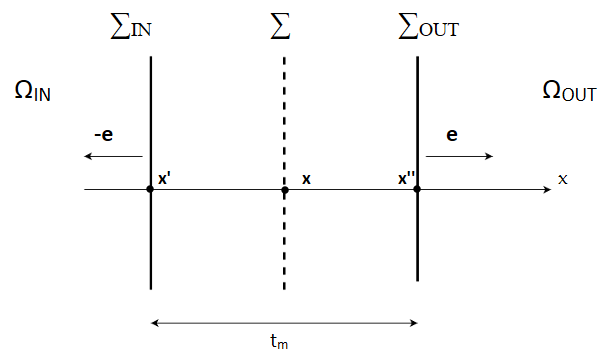
\includegraphics[scale=0.77]{intra.png} 
	\end{center} 
	\caption{\textit{Schematic model of a cellular membrane}}
	
\end{figure}

From a biological point of view, the different ionic concentrations, assumed inside and outisde the neuron, give rise to a \textit{passive transport} of ions, which moves accordingly to the \textit{electrochemical gradient} (i.e. movement of positive charges from high to low potentials). The passage of ion species across the membrane can be allowed or denied by \textbf{ionic channels}, each of one designed  for a specific ion. The passive trasnport is not the only mechanism of ionic transport. Indeed, thanks to special \textbf{ionic pumps}, the cell is able to perform an \textit{active} transport, moving ions against the electrochemical gradient. In order to do this, the cell needs to consume energy, in form of \textit{ATP}.\\
Let us consider a geometrical setting representing the relevant components of a neuron for its electrical activity: an intracellular region $ \Omega_{in}$ and an extracellular region $\Omega_{out}$. The two regions are separated by the cell's membrane, presenting internal and external surfaces $\Sigma_{in}$ and $\Sigma_{out}$. Finally, define the normal versors to  $\Sigma_{in}$ and $\Sigma_{out}$ as  $\textbf{n}_{in}$  and  $\textbf{n}_{out} = - \textbf{n}_{in}$.\\

Under this setting, we define the \textbf{total ionic current density} of ion $\alpha$ as

\begin{equation}
J_{\alpha,i}^{TOT} =	\textbf{J}_{\alpha,i}^{TOT} \cdot \textbf{n}_{i} = J^{cond}_{\alpha,i} + J^{cap}_{\alpha,i} \hspace{2cm} i= in,out
\end{equation}
	
	
The total current density is formed by two contributions:

\begin{itemize}
	
	\item \textbf{Conduction current} $J^{cond}_{\alpha}$: the current formed by the conudction of ions along the ionic channels. We assume no loss of current inside the channel, so that $J^{cond}_{\alpha, in} = J^{cond}_{\alpha, out}$
	
	\item \textbf{Capacitive current} $J^{cap}_{\alpha}$: the current formed by the charge accumulation in $\Sigma_{in}$ and $\Sigma_{out}$. The charge accumulation makes the membrane behave like a \textit{capacitor}. Thus, we assume 
	\begin{equation}
		J^{cap}_{\alpha,i} = \frac{\partial \sigma_{\alpha,i}}{\partial t}  \hspace{2cm} i= in,out
	\end{equation}
	
	where $\sigma_{\alpha,i}$ is the \textbf{surface charge density}. Also in this case we require \textit{wall's neutrality}
	
	\begin{equation}
\sigma_{\alpha,in} = \sigma_{\alpha,out}
	\end{equation}
\end{itemize}	
	
The neutrality conditions on conduction and capacitive current implies current conservation 

	\begin{equation}
	J_{\alpha,in}^{TOT} = J_{\alpha,out}^{TOT}
	\end{equation}
	
Considering two points $ \textbf{x}' \in \Omega_{in}$ and $ \textbf{x}'' \in \Omega_{out}$ and a time interval $ [0,T]$, we can consider the electric potentials $ \psi^{in} (t) = \psi(\textbf{x}',t) $ and  $ \psi^{out} (t) = \psi(\textbf{x}'',t) $, assuming the potentials constant respectively in $\Omega_{in}$ and $\Omega_{out}$. The \textbf{membrane potential} is then defined as

\begin{equation}
	\psi_m (t) = \psi^{in} (t) -  \psi^{out} (t) \hspace{1 cm}  t \in [0,T]
\end{equation}
	
	
	The existence of the membrane potential is consequence of the Faraday's equation (known as well as Maxwell's third equation)
	
	\begin{equation}
		\nabla \wedge \textbf{E} = -\frac{\partial \textbf{B}}{\partial t}
	\end{equation}
	
	where $\textbf{E}$ and $\textbf{B}$ are the elctric and magnetic field, respectively. In the microscopic cellular environment, it happens in practice that $ \left| \frac{\partial \textbf{B}}{\partial t} \right| << \left| \nabla \wedge \textbf{E}\right|$, being the magnetic contribution negligible qith respect tot he electric one. This implies from (2) that $\nabla \wedge \textbf{E} = 0 \implies \exists \psi s.t. \textbf{E} = -\nabla \psi$.\\
If $R_c$ and $t_m$ are, respectively, the cell's radius and the membrane's thickness, in practice we have that their ratio $ \eta_c := \frac{t_m}{R_c} << 1$. This implies that from a modeling point of view we can assume $t_m \sim 0 $, i.e. we can neglect the thickness of the membrane and assume $\Sigma_{in} \sim \Sigma_{out} \sim \Sigma$. In practice, for example, realistic values of such quantities can be $ R_c \sim 10^{-6} m$, $ t_m \sim 10^{-9} m$ and thus $\eta_c \sim 10^{-3}$.\\
If $\epsilon_m$ is the membrane's \textit{dielectric constant}, we can define the \textbf{specific capacitance} of the membrane as $ c_m = \frac{\epsilon_m}{t_m}$. Assuming then that the surface charge densities have the form $\sigma_{in}(\textbf{x}',t) = c_m \psi_m (\textbf{x},t)) $ and  $\sigma_{out}(\textbf{x}'',t) = -c_m \psi_m (\textbf{x},t) $, where $\textbf{x} \in \Sigma$. The capacitive current density (2) assumes the form

\begin{equation}
	J^{cap}_{\alpha,i}(\textbf{x},t) = c_m \frac{\partial \psi_m(\textbf{x},t)}{\partial t}  \hspace{1cm} t \in [0,T], \textbf{x} \in \Sigma
\end{equation}
	
	
\subsection{ODE local models}
	
	
\begin{figure}[H]
	\begin{center}
		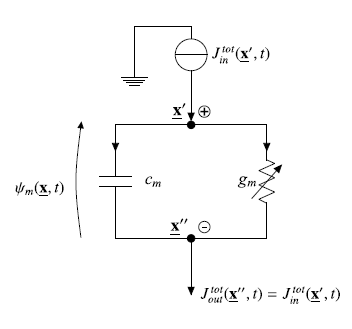
\includegraphics[scale=0.95]{ode_circuit.png} 
	\end{center} 
	\caption{\textit{Equivalent circuit of the total current density as in eq. (1)}}
	
\end{figure}
	
	Let us now consider a specific $\textbf{x} \in \Sigma$. Then, equation (1) expresses a balance law for the current densities $J_{\alpha,i}^{TOT}, i= in,out$, which can be divided in two contributed (capactive and conductive), where the capacitive current assumes the form $J^{cap}_{\alpha,i}(t) = c_m \frac{\partial \psi_m(t)}{\partial t}$.\\
	As for the conductive current, we consider a general form 
	
	
	
	
	
	
	
	
	
	
	
\end{document}
